\chapter{Additional Graphs and Tables}


\begin{figure}[h!]
	\centering
	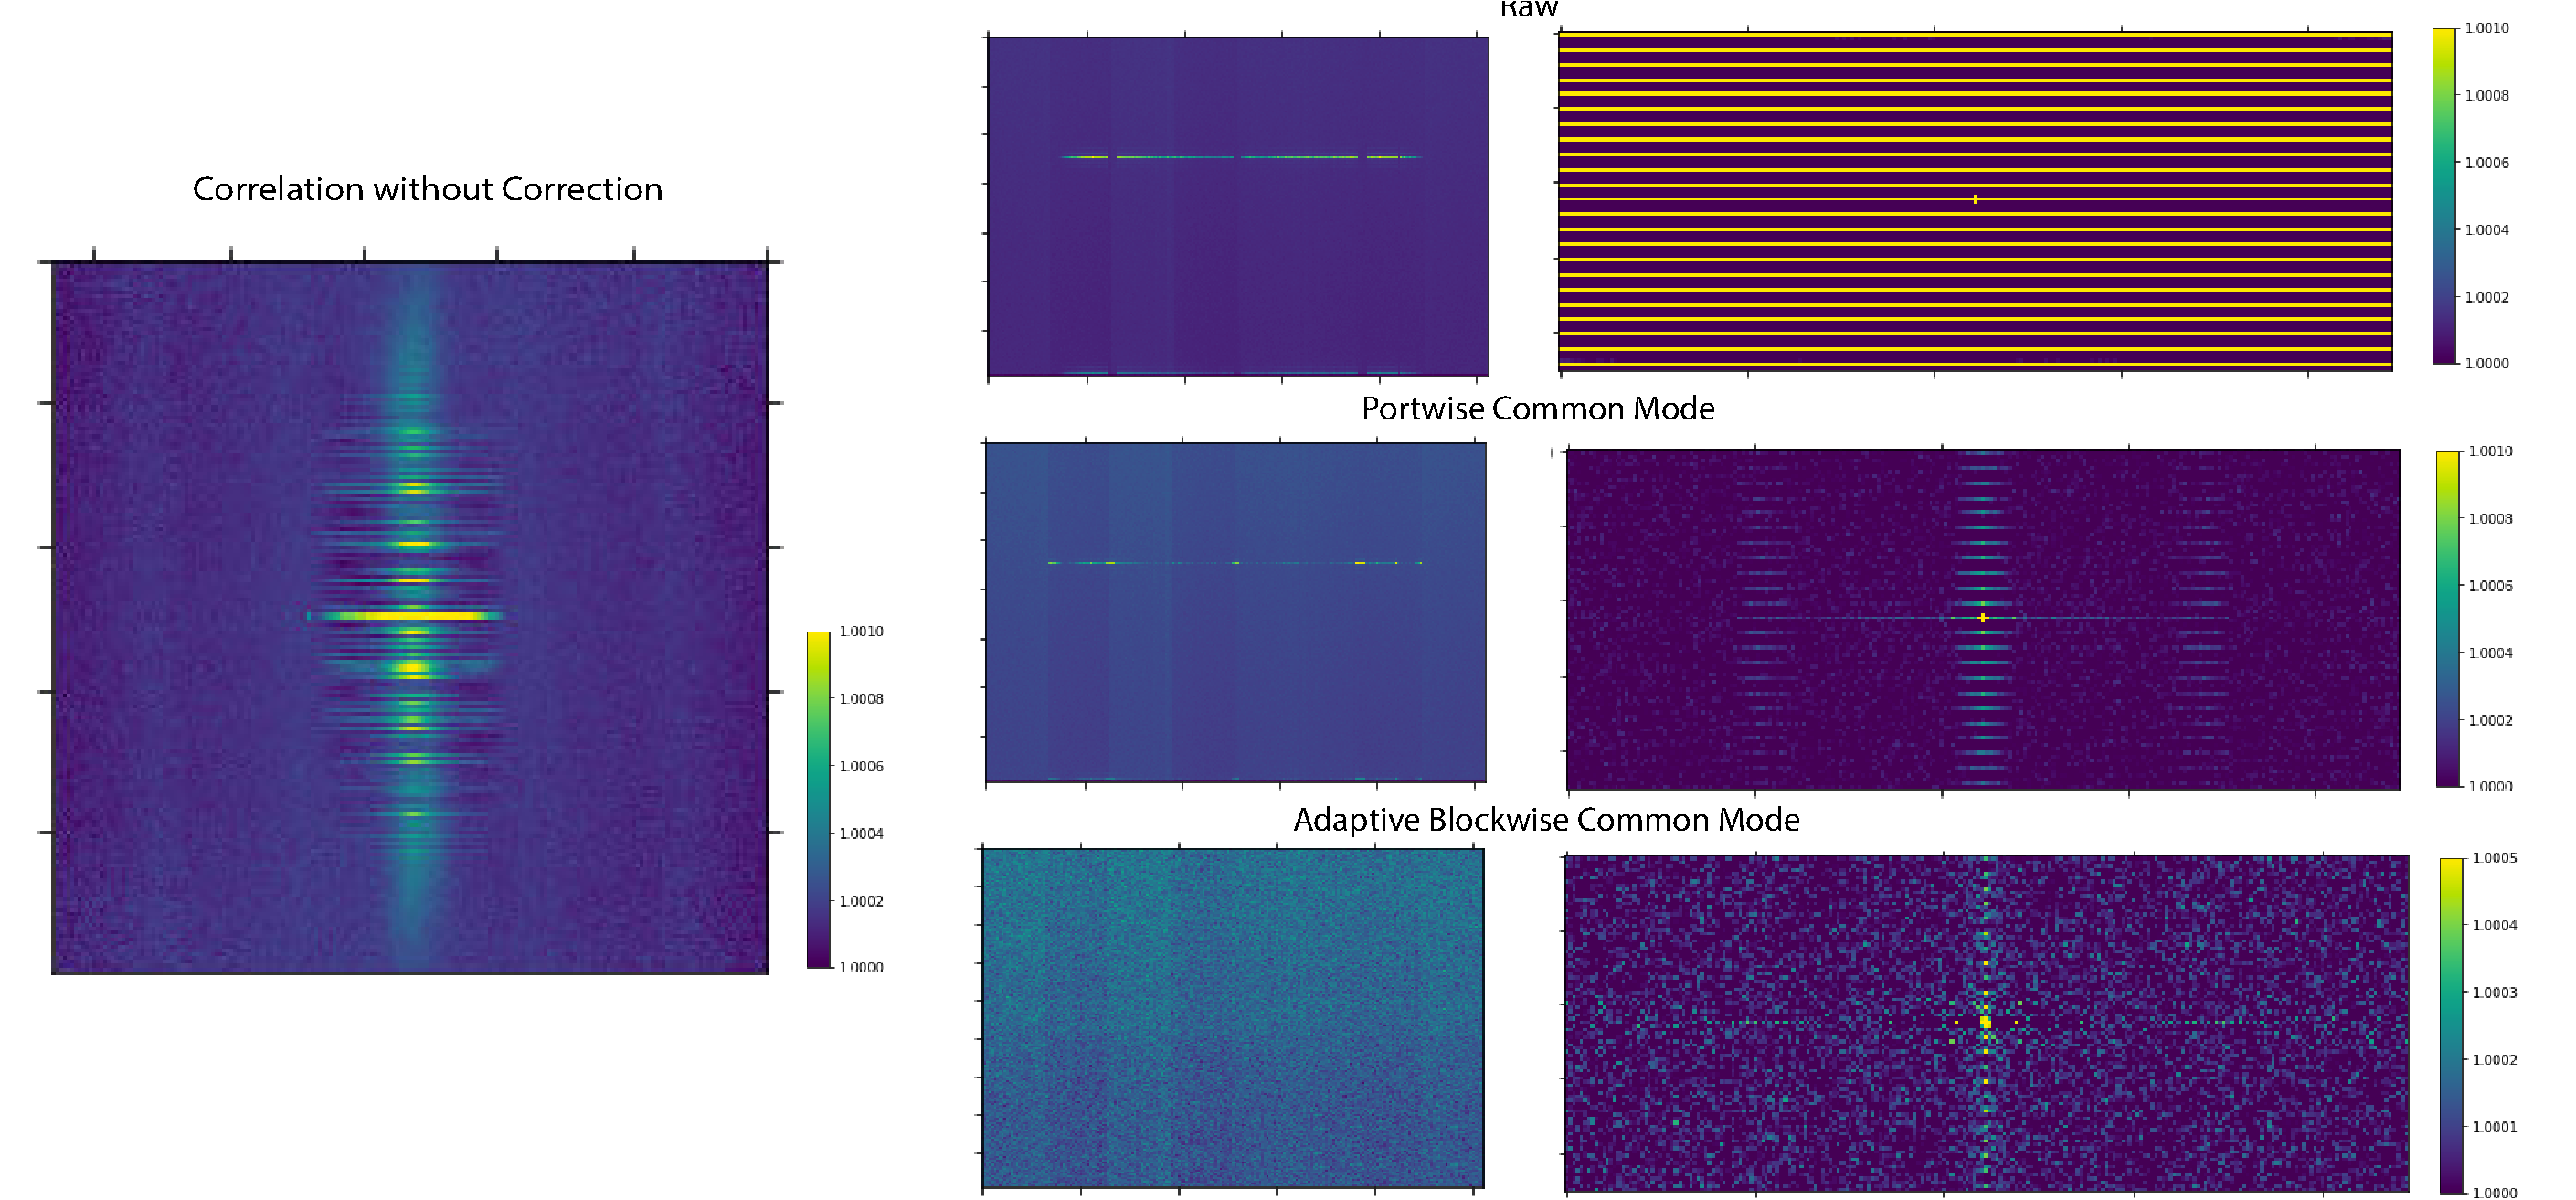
\includegraphics[width=\linewidth]{images/correction.pdf}
	\caption[Correction of periodic detector noise]{Correction of the periodic detector noise: On the left, the correlation without any applied correction for the periodic noise is shown. The artifacts occupy large areas of the reconstruction. On the right, the spatial spectrum for all columns of the detector and the center part of the correlation (right) are shown for three different cases: Raw (without the correction), with a portwise common mode correction using the median and a correction with adaptive blocks as described in the main text. The portwise correction creates artifacts on the non-affected columns of the detector, whereas the blockwise correction reduces the artifact to small areas that can easily be masked out.}
	\label{fig:app_correction}
\end{figure}

\begin{figure}[h!]
	\centering
	\begin{subfigure}[b]{0.32\textwidth}
		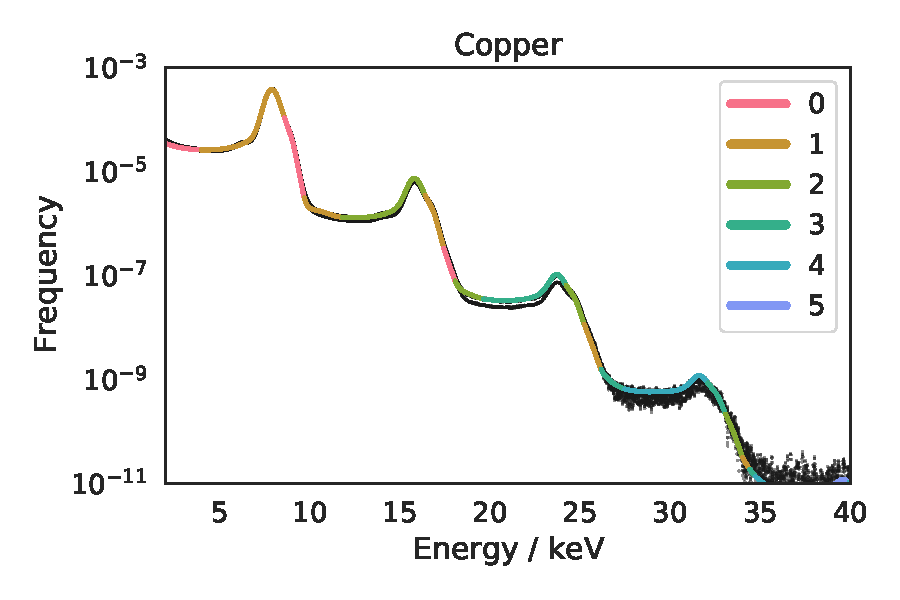
\includegraphics[width=\linewidth]{images/thresholdsCopperHighNoBeta.pdf}
	\end{subfigure}
	\begin{subfigure}[b]{0.32\textwidth}
		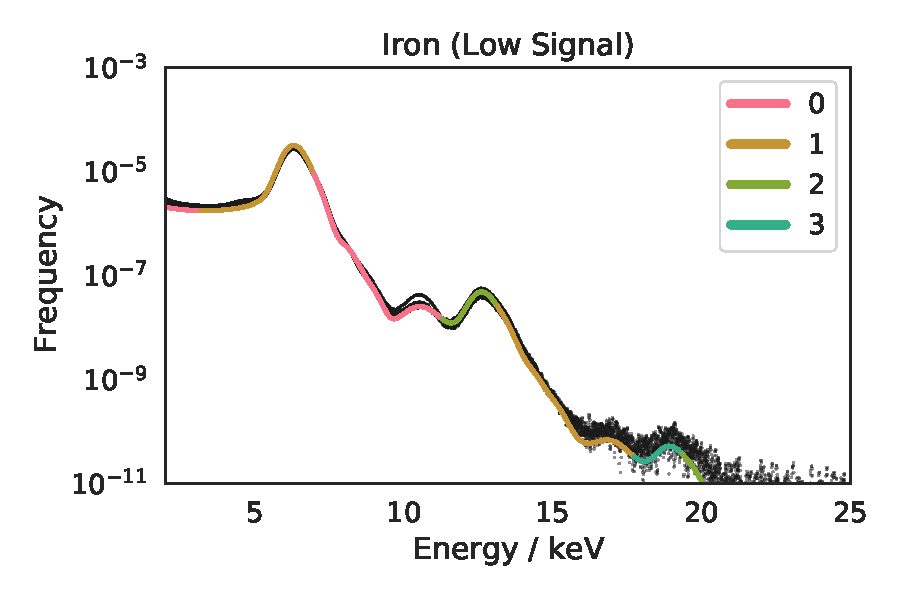
\includegraphics[width=\linewidth]{images/thresholdsIronLow.pdf}
	\end{subfigure}
	\begin{subfigure}[b]{0.32\textwidth}
		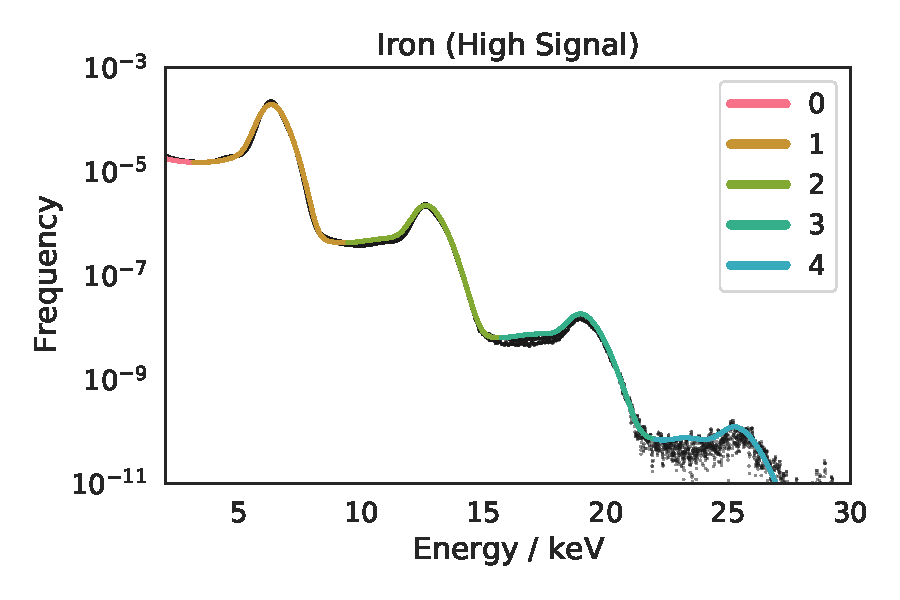
\includegraphics[width=\linewidth]{images/thresholdsIronHigh.pdf}
	\end{subfigure}
	\caption[Spectra of fluorescence using foil samples with photon number classes]{Spectra of fluorescence using foil samples (black), and spectra of the final regression models used for classification, colored by the assigned class of signal photon numbers. The initial values used for the regression are the average values found in the regression using approximated charge sharing, for the sharing width the estimation $\sigma\approx\frac{1}{6} \left(1-\sqrt{1-\rho }\right)$ is used.  The final values of the regression used for classification of photon events are show in \fref{tab:fitvalues}.}
	\label{fig:thresholdsfoil}
\end{figure}


\FloatBarrier
\begin{table}[h!]
	\centering
	\caption[Parameters for simulated spectra used to find thresholds]{Parameters for simulated spectra used to find thresholds. $E_{sig}$/$E_{scat}$ denote the energy of the signal/scattering background photons, $p_{sig}$/$p_{\beta}$/$p_{scat}$ the probability of a signal/K$_{\beta}$/scattering photons, $\sigma_{scat}$ the width (standard deviation) of the (approximated as Gaussian) scattering peak, $\sigma_{det}$ the standard deviation of (assumed as Gaussian) broadening due to detector noise and $\sigma_{sharing}$ the width of the charge sharing cloud.  As the $K_beta$ peak can be distinguished as a shoulder in the Copper spectra, $K_{\beta}$ is considered as noise there and treated like the scattering noise in the classification, resulting in tighter final thresholds ()resulting in partial rejection of  $K_{\beta}$) compared to counting those photons as signal.}
	\label{tab:fitvalues}
	\scriptsize
	\begin{adjustwidth}{-1em}{-1em}	
		\begin{tabular}{lrrrrrrrrrrrr}
			
			\toprule
			{} &  $E_{sig}$ &  $p_{sig}$ &  $p_{\beta}$ &  $E_{scat}$ &  $p_{scat}$ &  $\sigma_{scat}$ & $E_{scat,2}$ & $p_{scat,2}$ &  $\sigma_{det}$ &   M &  $\sigma_{sharing}$ &  $K_{\beta}$ as noise \\	\midrule
			Copper &          7940 &       4.7e-02 &     1.5e-01 &          10500 &        5.0e-05 &                 450 &           8150 &        5.9e-05 &             350 &  20 &             4.2e-02 &                  True \\
			Iron High         &          6340 &       2.5e-02 &     1.5e-01 &          10700 &        1.5e-05 &                 500 &                &                &             420 &  20 &             3.5e-02 &                 False \\
			Iron Low          &          6320 &       3.3e-03 &     1.5e-01 &          10570 &        3.0e-06 &                 380 &           8000 &        3.7e-05 &             350 &  20 &             3.0e-02 &                 False \\
			\bottomrule
		\end{tabular}
	\end{adjustwidth}
\end{table}


\begin{figure}
	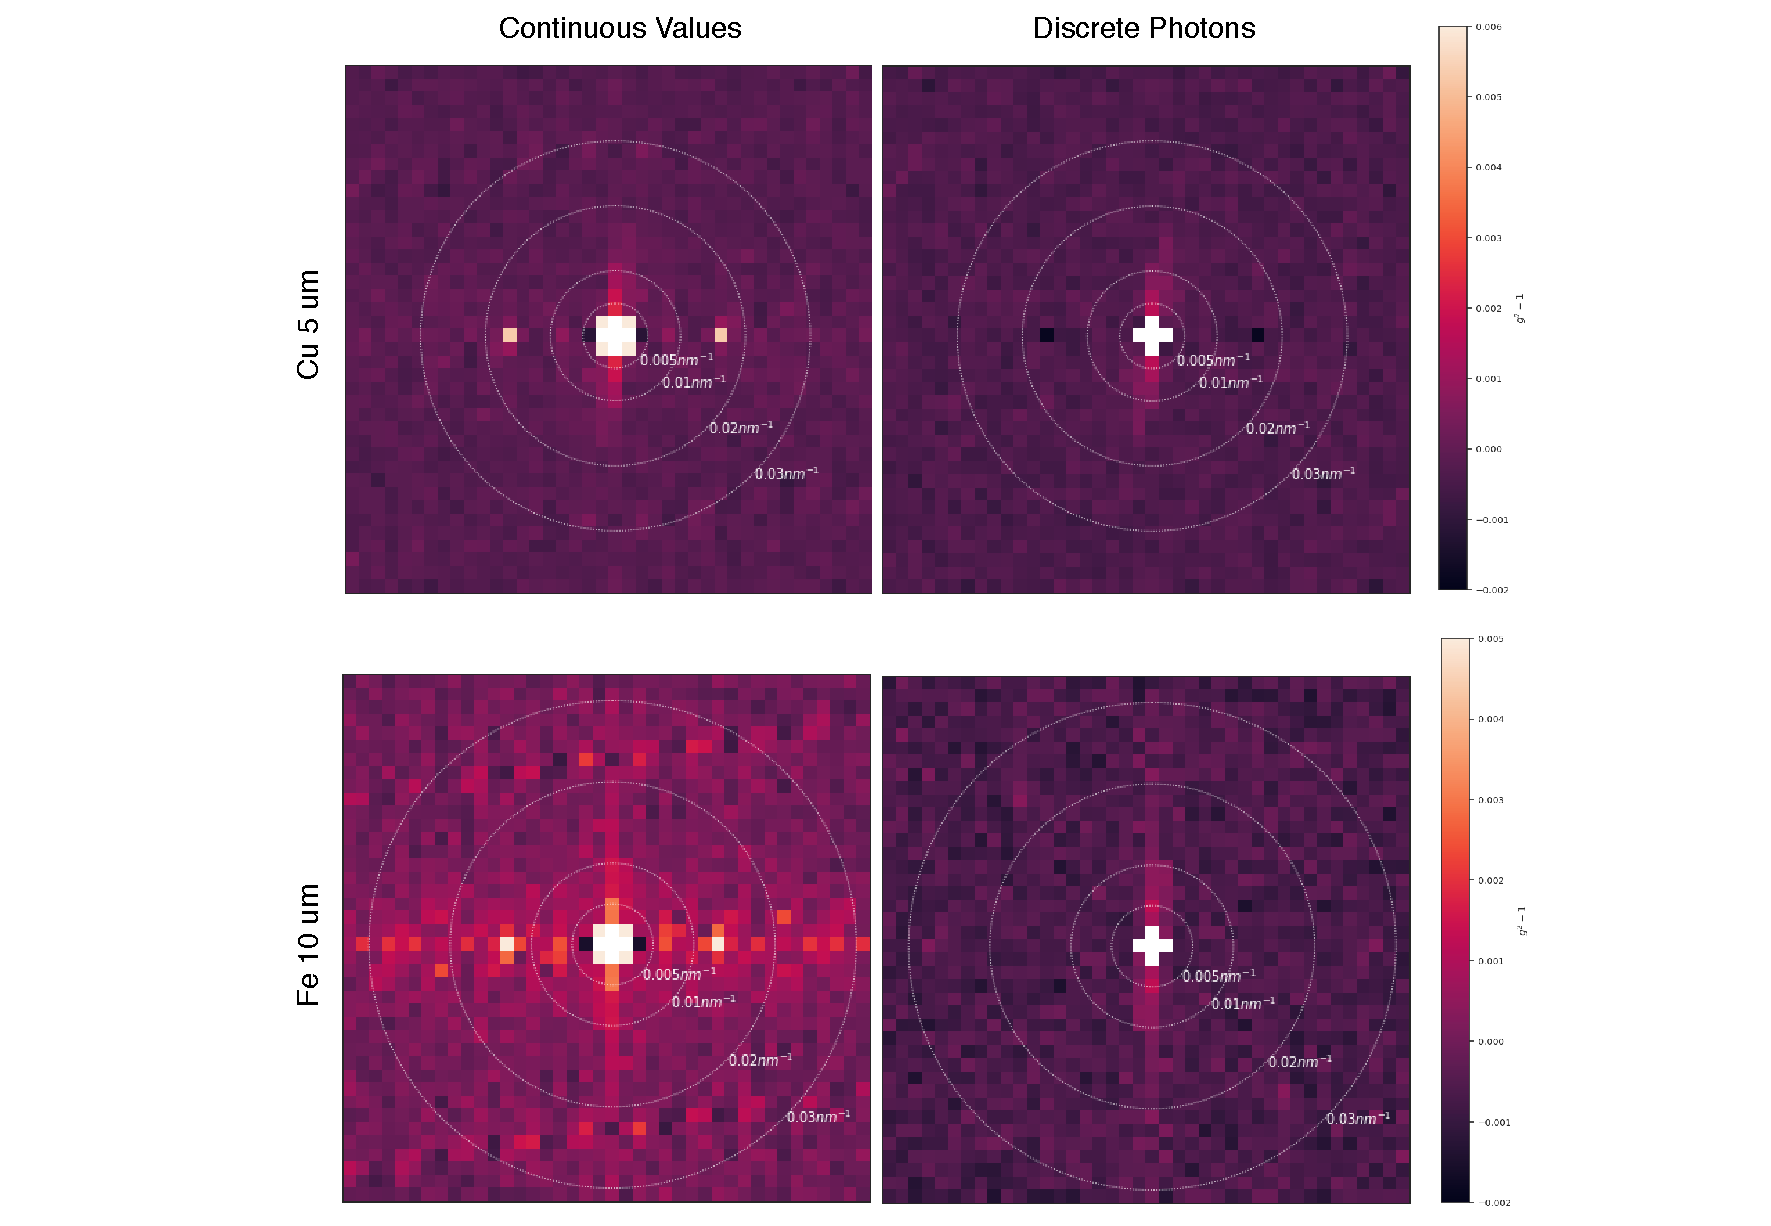
\includegraphics[width=\linewidth]{images/foil_photonmodes.pdf}

	\caption[Effect of discretizing the signal into photons]{Effect on the reconstruction of discretizing the signal into photons: For two foils at focal position,  correlations of the thresholded, continuous energy values as well as correlations after discretizing into photons are shown. Artifacts caused by charge sharing (for example diagonally neighboring pixels being correlated, visible as a square in the center) and other detector imperfections are greatly reduced by discretizing.}
	\label{fig:foil_photonmodes}
\end{figure}

\begin{figure}
	\centering
	\begin{subfigure}[b]{0.49\textwidth}
		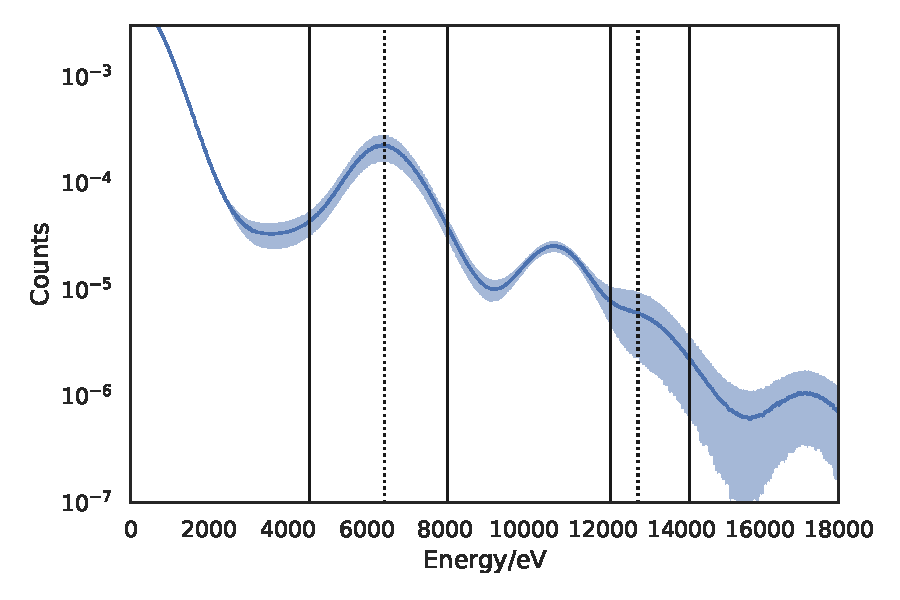
\includegraphics[width=\linewidth]{images/spectrum_nano.pdf}
			\caption {10\,nm NP in PS}
			\label{fig:spectrum_nano}
	\end{subfigure}
	\begin{subfigure}[b]{0.49\textwidth}
		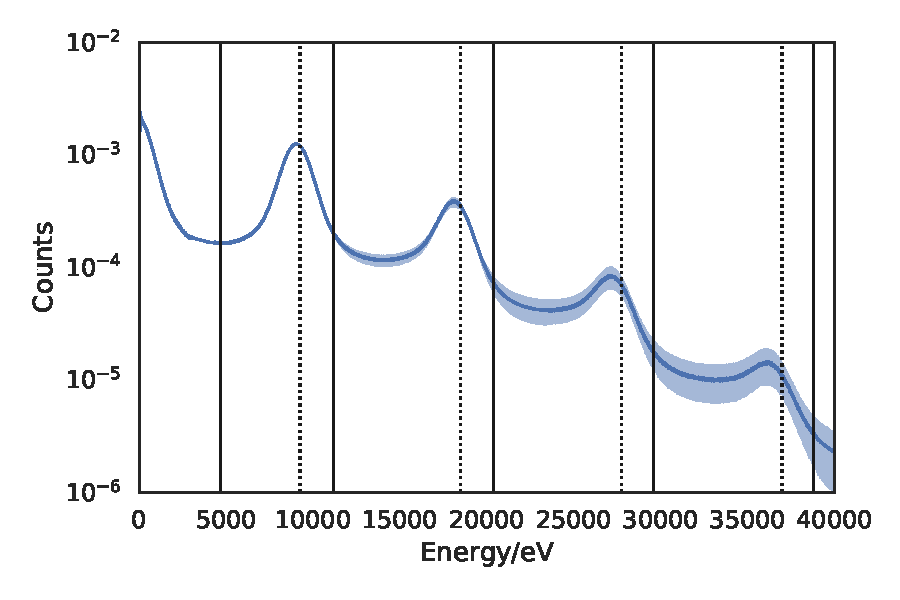
\includegraphics[width=\linewidth]{images/spectrum_gaas1.pdf}
		\caption{GaAs Sample 1}
		\label{fig:spectrum_gaas}
	\end{subfigure}
	\caption[Spectrum on the detector for nanoparticle and  GaAs samples]{The histogram of the energies recorded by the octal detector after applying all corrections and filtering in counts per images and pixel per 10\,eV bin  The dashed lines are multiples of the iron/gallium K$_\alpha$ energy, the black lines signify the thresholds for the different numbers of signal photons, the colored band shows the standard deviation over different shots. As the nanoparticle sample produces only $\approx 0.04$ signal photons per shot and image and no filter is used, the scattering peak at 11\,keV is higher than the two-photon fluorescence peak.}

\end{figure}

\begin{figure}[h!]
	\centering
	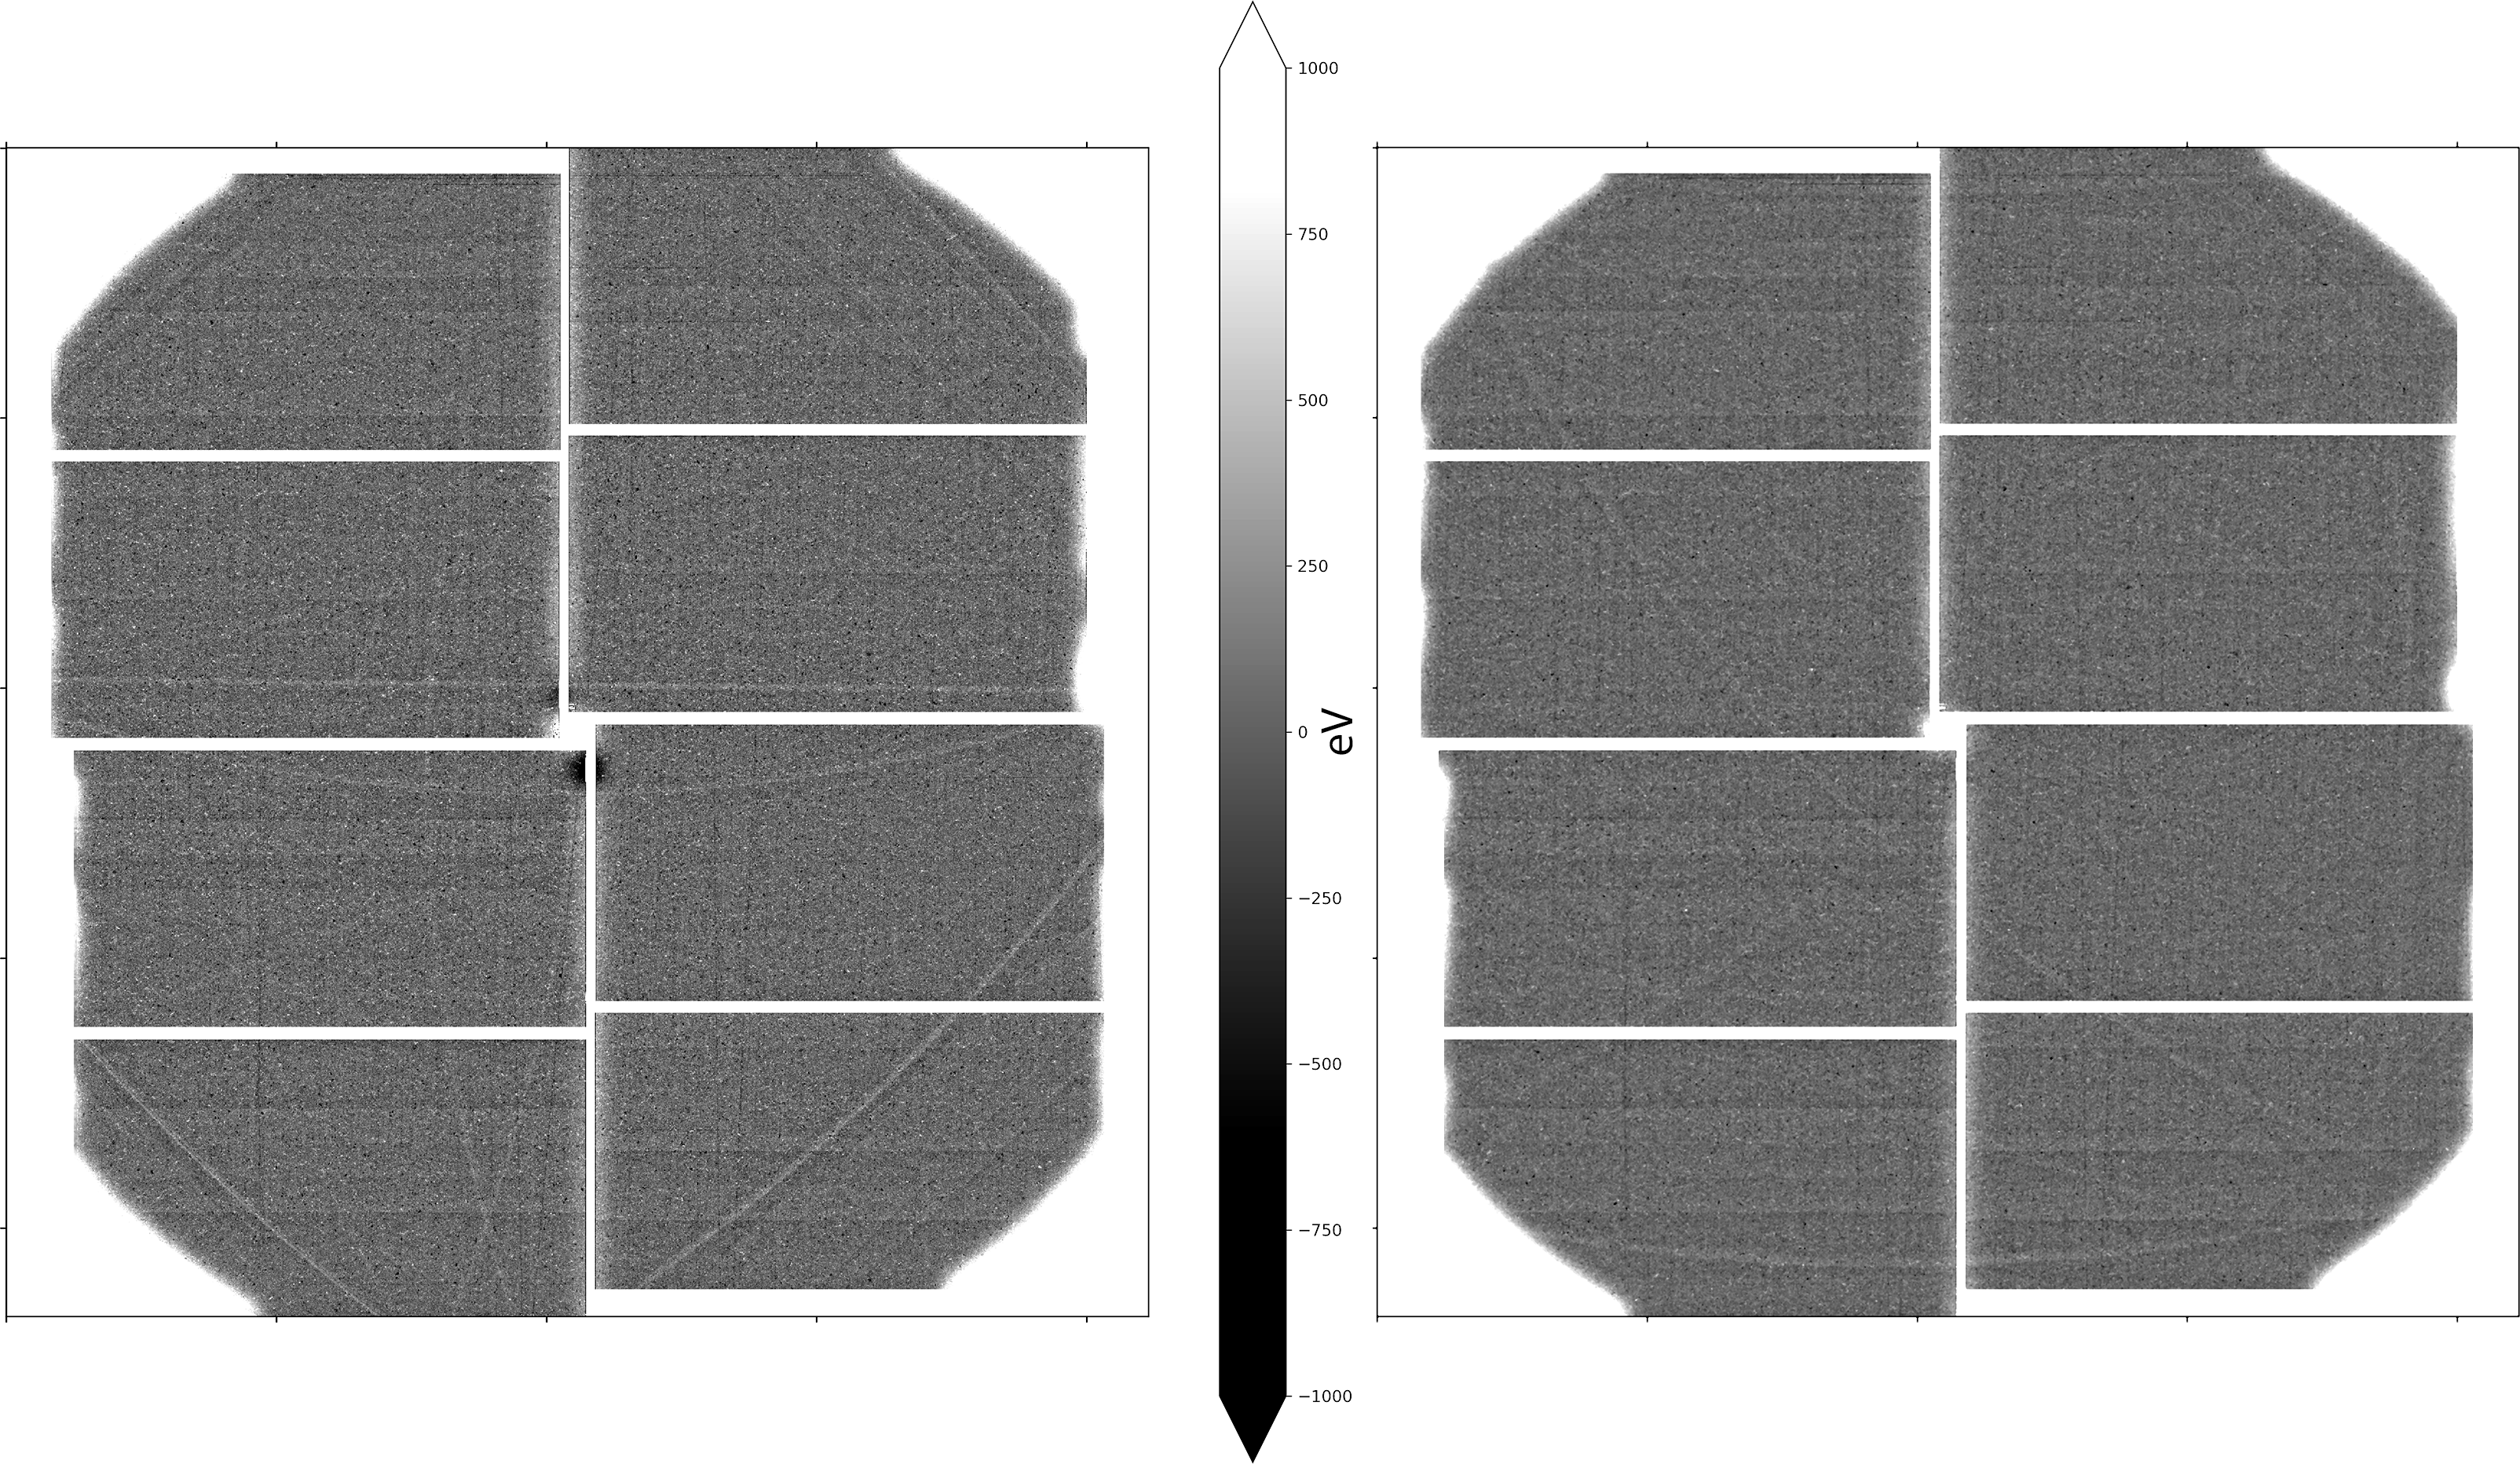
\includegraphics[width=0.8\linewidth]{images/kossel_gaas.png}
	\caption[Mean image of fluorescence of GaAs after background subtraction with visible Kossel lines ]{Mean images of 5000 shots after background subtraction for sample 1 (left) and sample 2 (right), showing the (faint) Kossel lines and some artifacts at the edges.}
	\label{fig:kosselgaasmean}
\end{figure}



\begin{table}[hp!]
	\caption[Miller Indices considered in Kossel line least squares regression of GaAs sample]{Miller Indices considered in Kossel line least squares regression of GaAs sample 1 (left) and sample 2 (right). Not all possible Kossel lines are visible in the recorded images.}
	\label{tab:kosselpeaks}
	\begin{tabular}[t]{lll}
		\toprule
		h&           k &        l \\
		\midrule
	 1 & -1 &  1 \\
	-1 &  1 &  1 \\
	-1 & -1 &  1 \\
	2 & -2 &  0 \\
	-2 &  2 &  0 \\
	-2 & -2 &  0 \\
	2 &  2 &  0 \\
	-3 & -1 &  1 \\
	3 &  1 &  1 \\
	-1 & -3 &  1 \\
	2 & -2 &  4 \\
	-2 & -2 &  4 \\
	2 &  2 &  4 \\
	-2 &  2 &  4 \\
	-4 &  0 &  4 \\
	0 &  4 &  4 \\
	4 &  0 &  4 \\
	0 & -4 &  4 \\
				\bottomrule
	\end{tabular}
\hspace{1cm}
	\begin{tabular}[t]{lll}	
	\toprule
	h&           k &        l \\
	\midrule
 2 &  2 &  0 \\
-2 &  2 &  0 \\
2 & -2 &  0 \\
0 & -2 &  2 \\
0 &  2 &  2 \\
2 &  0 &  2 \\
-2 & -2 &  0 \\
-2 &  0 &  2 \\
-3 & -1 &  3 \\
-1 & -3 &  3 \\
1 &  3 &  3 \\
3 &  1 &  3 \\
-1 &  3 &  3 \\
1 & -3 &  3 \\
0 & -4 &  4 \\
-4 &  0 &  4 \\
0 &  4 &  4 \\
4 &  0 &  4 \\
0 &  2 &  6 \\
2 &  0 &  6 \\
-2 &  0 &  6 \\
0 & -2 &  6 \\
	\bottomrule
\end{tabular}
\end{table}





\begin{figure}[hp!]
	\centering
	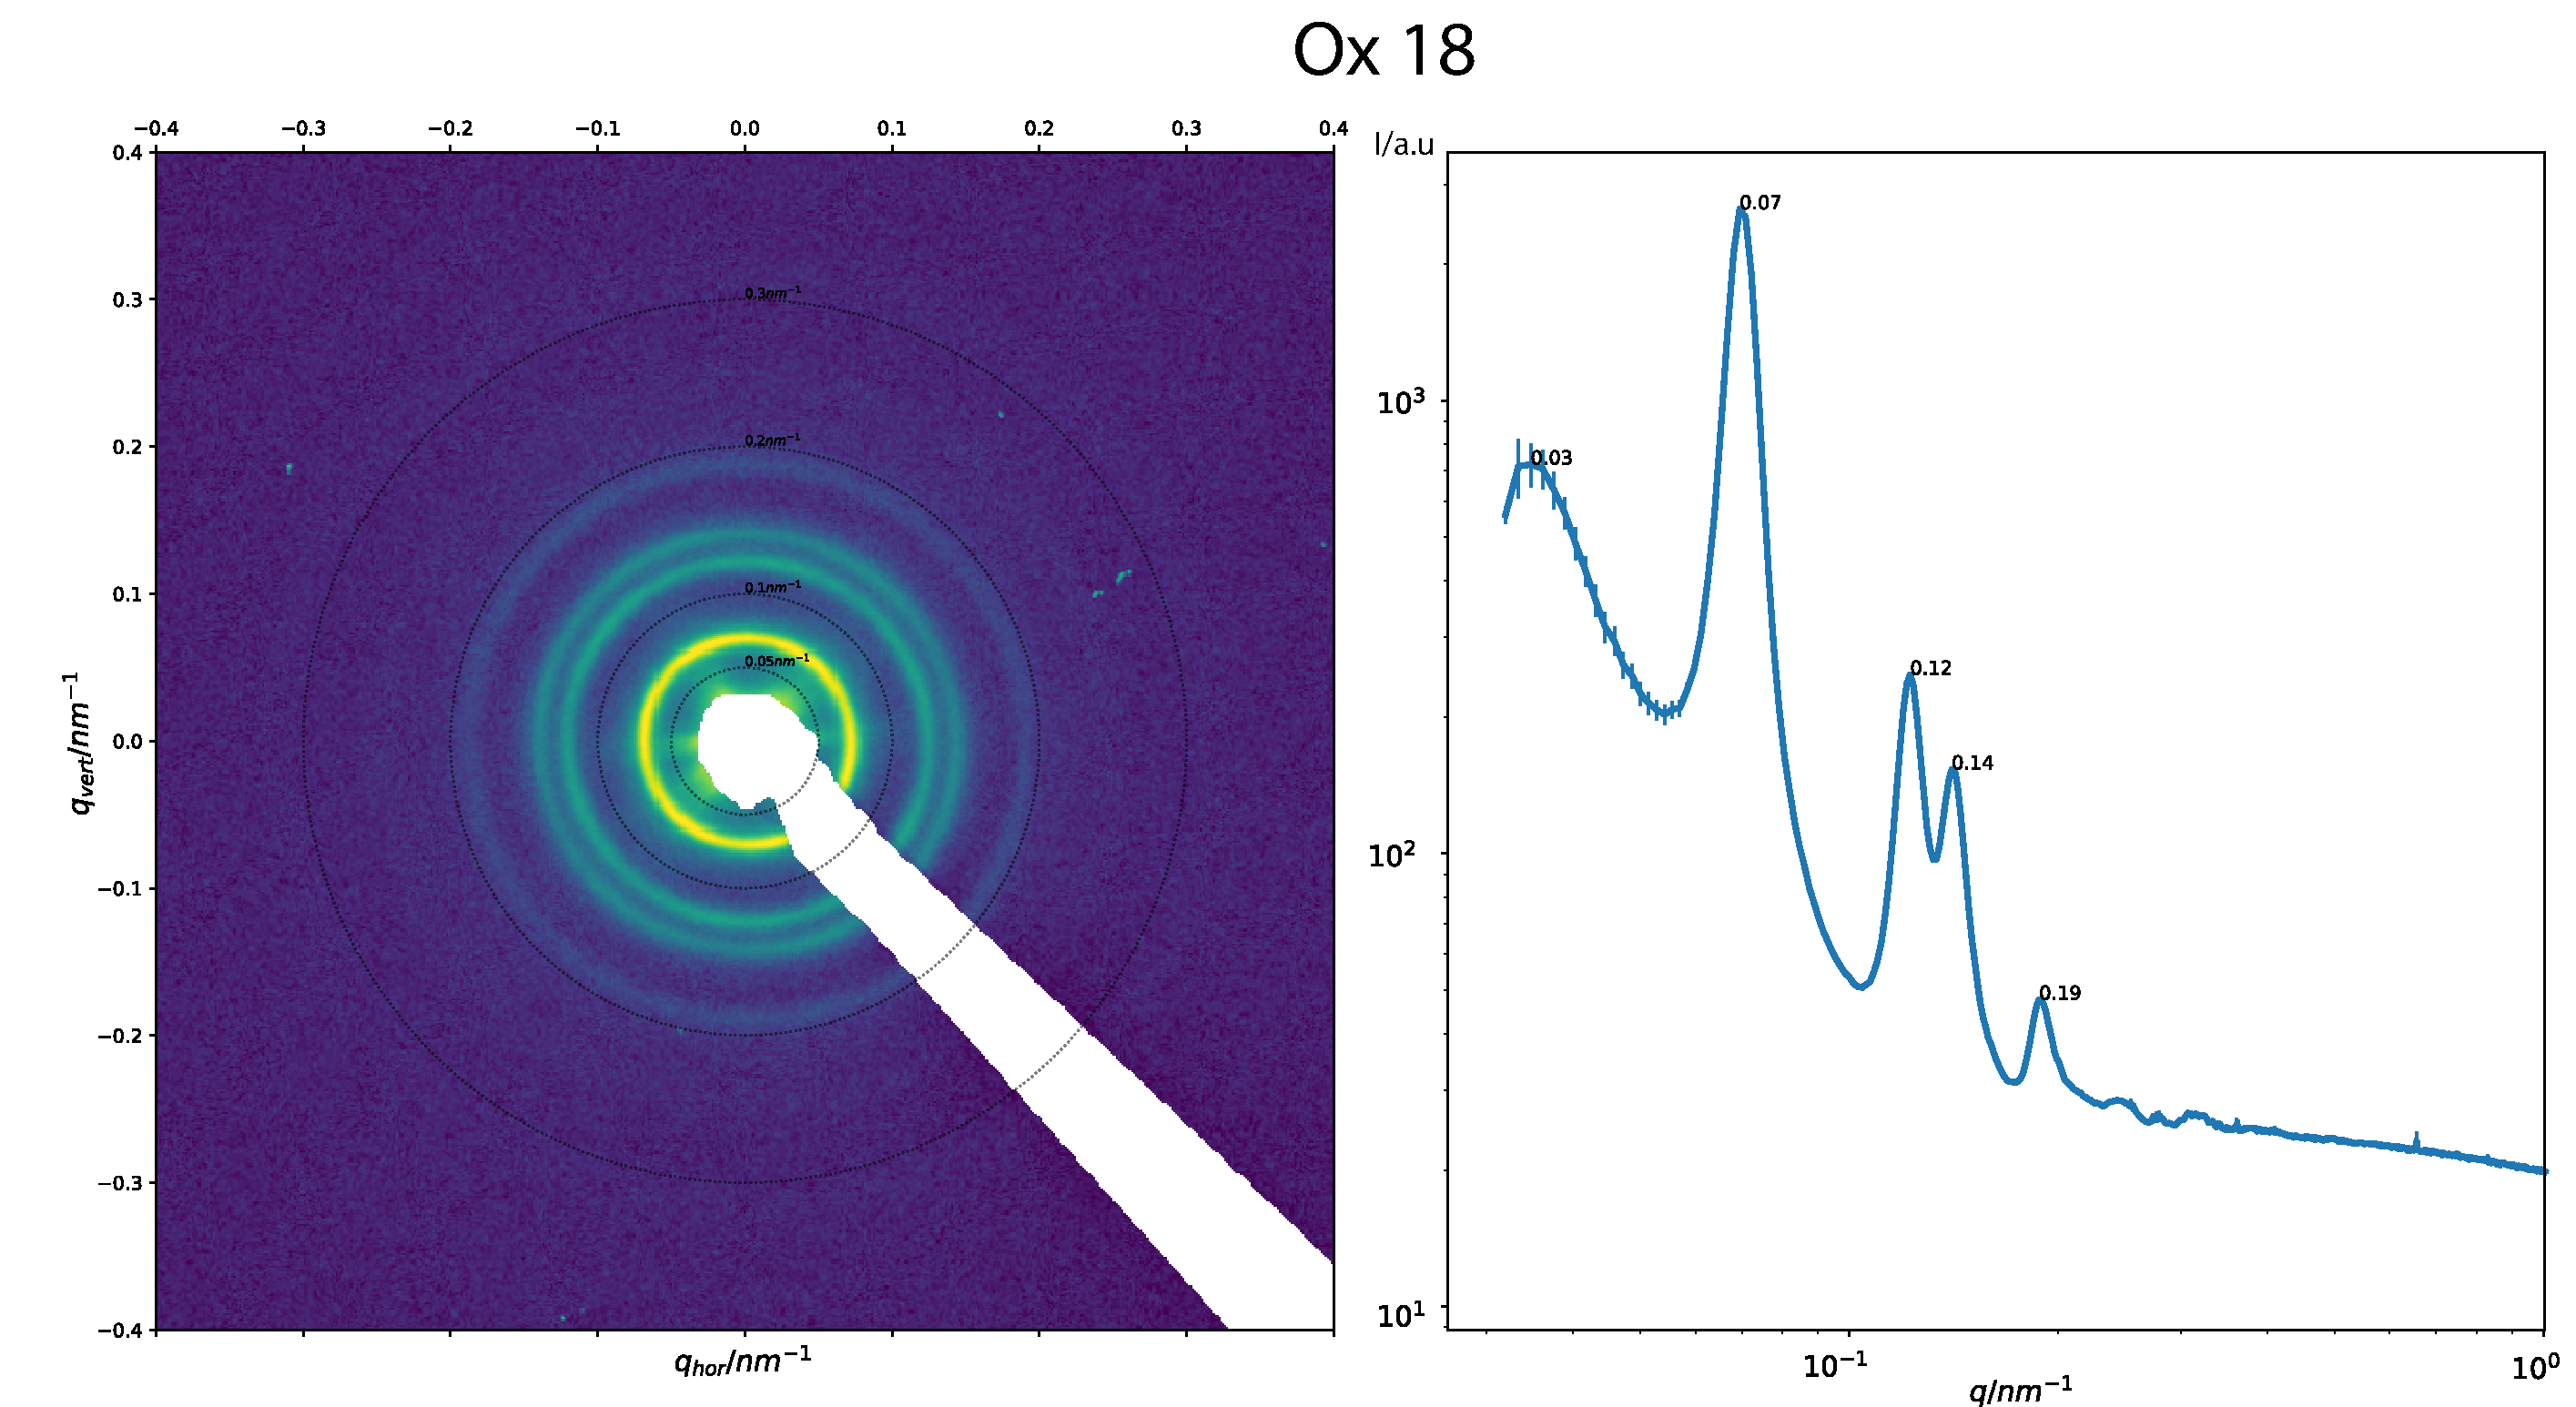
\includegraphics[width=0.8\linewidth]{images/ox18.pdf}
	\caption[SAXS of AAO membrane sample]{SAXS measurement of one of the AAO membranes used for the LCLS experiment, showing well defined features which can be used in an IDI measurement.}
	\label{fig:saxsaao}
\end{figure}



